\documentclass{acm_proc_article-sp}

\usepackage{graphicx}
\graphicspath{ {images/} }

\begin{document}

\title{Subway Spot Selection}
\subtitle{A Behavioral Model}

\numberofauthors{1} 
\author{
\alignauthor
       Dan Gopstein\\
       \affaddr{New York University}\\
       \email{dgopstein@nyu.edu}
}

\date{December 2014}


\maketitle
\begin{abstract}
We introduce a behavioral model of the subway passenger that describes their spot selection process upon on boarding the train car. We propose that passengers choose their spot based on a mixture of environmental and social factors. We go on to analyze the social optimization problem as a resource selection game.
\end{abstract}

\section{Introduction}
The New York City Subway system provides, on average, over 5 million rides every weekday~\cite{MTAFacts}. The interior design of subway cars has a daily impact on millions of urban commuters. Subway car utilization is an important factor in public transit ecosystem of many large cities. Previous work has focused on observational studies of topics from spot selection\cite{berkovich2013observed} to physiological reactions\cite{evans2007crowding} to race\cite{maines1979ecological} and sex\cite{hai1982sex} issues. Relatively less researched have been the underlying models that humans use to make these decisions. Through observational data (kindly provided by Alex Lu of Berkovich, Lu, Levine, Reddy), user studies and intuition garnered from psychological research\cite{evans2007crowding, hai1982sex, maines1979ecological} we have created and validated a computational model of the subway passengers decision making process. Using this model we then translate the human value system into an objective function that we use in an economic model based off techniques in resource selection.

[Describe the "Spot Selection Game"]

\section{Data}
Before developing an accurate economic model of the Spot Selection Game, we first had to understand the factors that motivate the passengers themselves. There were two major data sets used in generating our model. First, were the observed passenger data from Berkovich, et al. Second were responses from a survey that we designed to help understand which design factors were important when passengers made their spot selection.

\subsection{Observed Passenger Data}
The most significant data set used to build the decision model was that provided by Berkovich, et al. Their team rode subway cars and manually annotated forms describing the positions of each sitting and standing passenger on subway cars for individual stops along several routes. For a more thorough description of their methods, see their report\cite{berkovich2013observed}. In total they recorded 1925 passenger positions for 62 stops, over 45 stations, on 15 lines, in 11 classes of car. In our usage of of Berkovich, et al's data, there are some situations such as inferring patterns where we used the entire data set, and other situations, such as verifying the results of our simulations, where we only used data from the single most heavily observed car class, the R68, for which 14 stops' passengers were observed.

\subsection{Decision Motivation Survey}
In order to inform the design of our passenger decision model, we solicited descriptions of 12 subway passenger's own thoughts on where they choose to sit or stand, and why they made those decisions. The survey was broken up into two sections. First, the participants were asked rank, in order of preference, which seats or standing positions they preferred on a given subway car. Then, they were asked to describe which factors most influenced their decision to sit or stand, and about their relative preference stand versus sit when possible.

Participants were asked for a freeform response to the question "When you decide to sit on the subway, which factors matter in selecting which seat to sit in?". By hand, we analyzed the responses aggregating commonly cited motivation. The most commonly mentioned factor that influences seating location was, as one participant phrased it "closeness to other people". 2/3rds of all participants listed avoiding proximity to others as an important factor in their decision process. 1/2 of all participants cited distance from the door as a undesirable quality for a seating location. 5 people claimed that in certain cases standing was actually preferred over sitting. Other comments that were listed less frequently, or with less emphasis were complaints such as "minimize contact with w/all surfaces", "facing forward", "I won't sit to give women \& elderly space to sit", "leg room is a large consideration because of my height", "Is the person I'd sit next to a junky, pervert or someone abnormally smelly?"

\begin{figure}[h!]
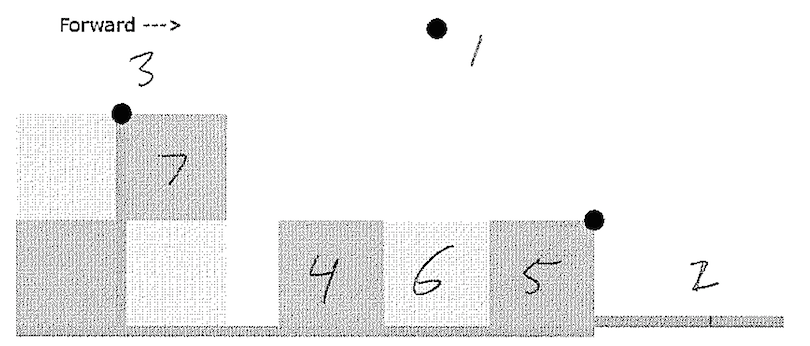
\includegraphics[width=\linewidth]{survey_response}
\caption{An example response from the seat chart portion survey. This passenger prefers to stand, then prefers the non-middle longitudinal seats.}
\end{figure}

\section{Simulation}
Our self report data was designed specifically to illustrate the qualitative thought processes involved in the spot selection problem. Since our eventual goal in this study was to generate a quantitative model of the decision making process we had to then go further and design interactive experiments. Due to logistical concerns, staging experiments in a real subway car with real passengers was out of the question. Instead we opted to develop a software model of the subway passenger and run simulated trials against our observed data.

\subsection{Modeling the environment}
The subway ecosystem, like many real-world environments, have to many incidental variables to make an intuitively interesting model. We tried to abstract the subway system as much as possible while retaining the salient details for the problem at hand. At the center of our simulation was the subway car itself. The designs of the cars in our study were taken directly from the descriptions used in data acquisition from Berkovich, et al. In their model the subway car floor plan is discretized into a grid of 1 person by 1 person squares, each representing either a seat or standing space (or inaccessible region, such as the conductors booth). Each square on the grid maybe occupied by exactly 0 or 1 persons, in our model crowding effects do not influence personal space beyond that level of granularity. Given our somewhat limited data, aside from one or two experiments testing differences between males and females, we did not segment passengers and generated only a single model which represents the thought process of an average individual. On- and off-boarding of passengers was modeled as closely as possible to our observed data, but since the data did not specify which doors passengers arrived from, we chose to assume that each passenger came in through the nearest door. This assumption is obviously false occasionally, but the resultant simulation based on learning from this assumption did still exhibit the behavior of walking as far as necessary to satisfy the simulated passenger if other factors seemed more pertinent than distance from the entrance door. In real life passengers exiting a train car and new passengers entering must both negotiate for right of way through the car door. In our simulation we limit the effects of these traffic jams in several ways. First we instantly off board all exiting passengers, they don't "exit", they just vanish. Secondly, all on boarding passengers are serialized, each passenger gets a turn to select their seat without fending off other passengers. Thirdly, passengers do not have to walk past other passengers, a cluster of people standing by the door does not hinder progress to the center of the train. We also assumed that once a passenger chose their spot they would not move for the duration of their trip. This assumption is fairly accurate for seated passengers, however it breaks down for standing passengers who tend to move often as passenger flow through the walkways pushes them about. Finally, we neglect the influence of load factor on the passenger's model. It is entirely likely that people's strategies change with respect to the total number of people on the train. Specifically, Berkovich, et al. note that passengers' willingness to sit is a non-linear function of train density.


\section{Results and Discussions}
Through user studies, surveys and predictive modeling we developed an object that mimics the behavior of passengers on the R68 subway car.

\bibliographystyle{abbrv}
\bibliography{subway}

%\balancecolumns 

\end{document}
